% • Problem and motivation of the work (rather short repetition)
% • Research questions (rather short repetition)
% • Problem analysis (rather short repetition)
% • Approach and solution to the problem
% • Evaluation of the solution
% • Distinction from and advancement beyond related work
% • Final conclusion

\section{Motivation}
\begin{frame}
    \begin{figure}
        \centering
        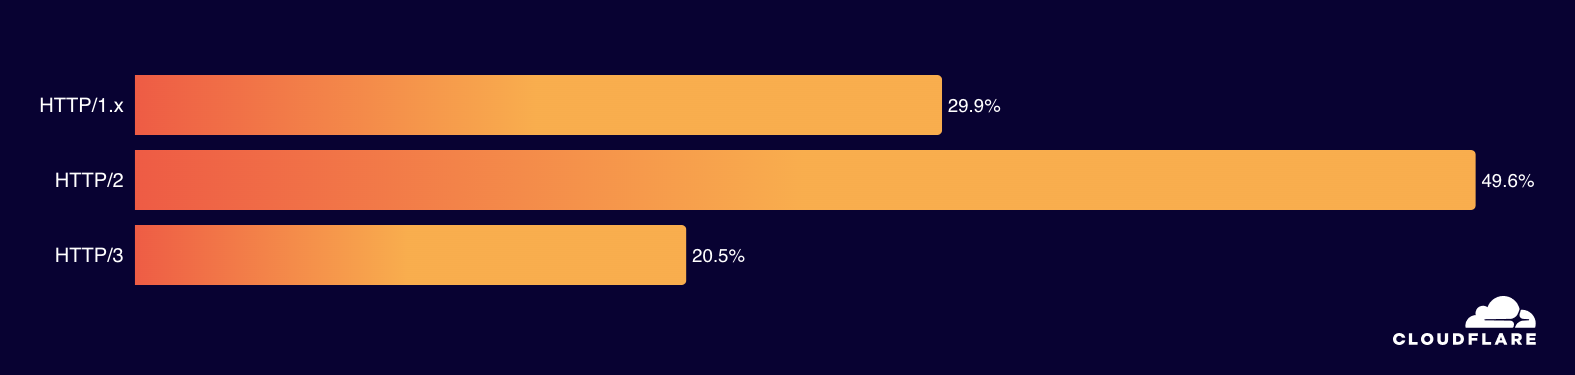
\includegraphics[width=.95\textwidth]{pics/http3-usage-cloudflare.png}
    \end{figure}
    \begin{itemize}
        \item Roughly 20\% of the world's internet traffic now runs on HTTP/3, the protocol built on QUIC\footnote{https://radar.cloudflare.com/year-in-review/2024\#http-versions}\nocite{cloudflare2024}
        \item QUIC throughput is not able to match TCP with increasing bandwidth\footnote{Zhang et al., Quic is not quick enough over fast internet, WWW ’24, pp. 2713–2722}\nocite{Zhang_2024}
        \item Packet I/O is the largest bottleneck for major QUIC implementations in terms of its maximum achievable goodput\footnote{Jaeger et al., Quic on the highway, June 2023, pp. 1–9.}\nocite{quic_on_the_highway}
        \item Work has been done to address this bottleneck: DPDK, Linux-in-QUIC, and Generic Receive Offload (GRO) with Generic Segmentation Offload (GSO).
    \end{itemize}
    \begin{center}
        \textbf{XDP offers an additional approach}
    \end{center}
\end{frame}

\section{Research Questions}
\begin{frame}
    \begin{itemize}
        \item To what extent can we increase QUIC performance by using XDP in a trivial way? Is there optimization potential?
    \end{itemize}
    \begin{itemize}
    \item Can a taxonomy be created for QUIC optimizations, categorized by:
        \begin{itemize}
            \item Implementation complexity
            \item Performance improvement potential
            \item Unwanted side effects
            \item Privilege level usage
            \item Deployment
        \end{itemize}
    \end{itemize}
\end{frame}

% - Start off by talking about motiviation
%     - HTTP/3 commands 20\% of internet traffic worldwide and projected to grow? (this is why it's important)
%     - It has been shown to be slower than TCP on high-bandwidth networks (the problem)
%     - So we have to figure out a way to make it faster
%     - The biggest bottleneck in QUIC is packet I/O
%     - So let's explore one of the ways to reduce packet I/O -- i.e. XDP

\section{XDP Primer}
\begin{frame}
    \begin{itemize}
        \item XDP is a native Linux hook point for eBPF bytecode to run in
        \item Decide on an action for each packet: \texttt{XDP\_DROP}, \texttt{XDP\_PASS}, \texttt{XDP\_REDIRECT}, \texttt{XDP\_ABORTED}, \texttt{XDP\_TX}
    \end{itemize}
    \begin{figure}
        \centering
        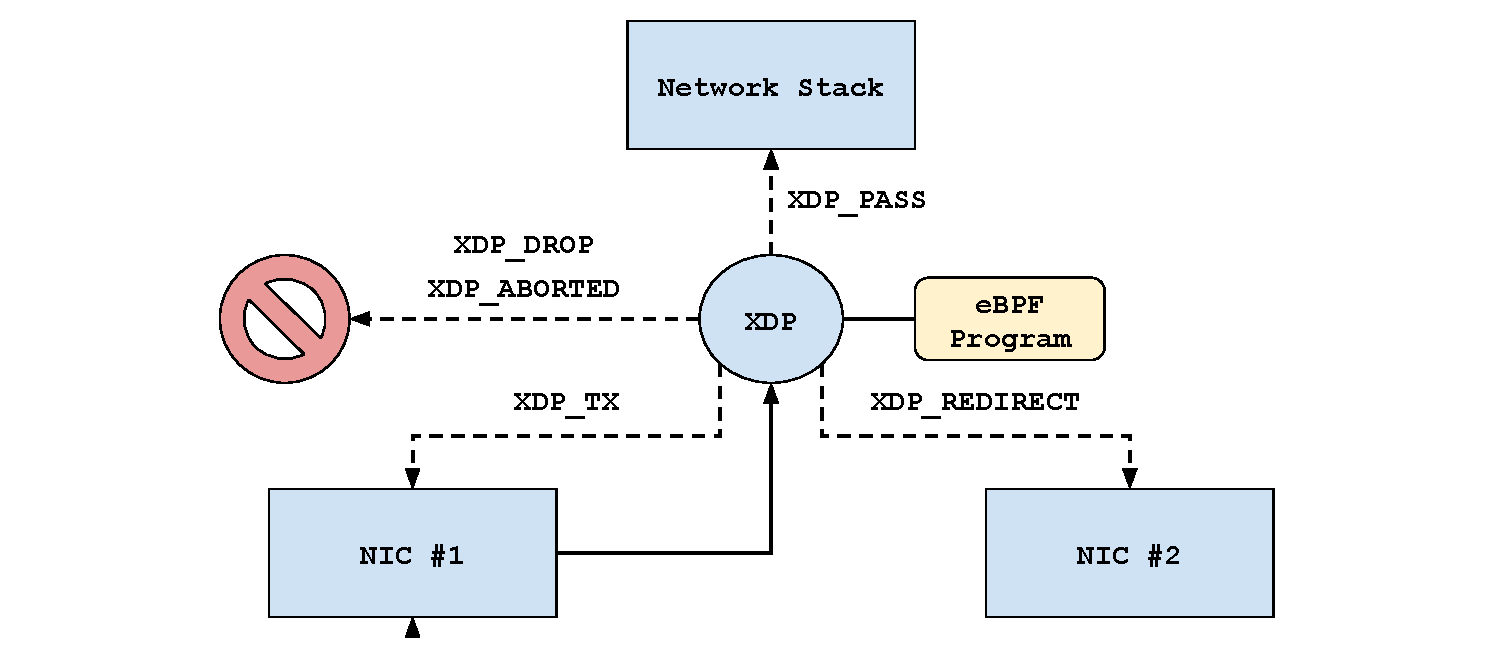
\includegraphics[width=.90\textwidth]{pics/xdp-actions2.pdf}
    \end{figure}
\end{frame}

% NOTES:
% - Represents one of the earliest points the OS can access a packet

\section{XDP Primer}
\begin{frame}
    \begin{itemize}
        \item AF\_XDP is an address family in Linux similar to AF\_INET or AF\_INET6
        \item Works with XDP to bypass the network stack 
        \item Helps avoid costly per packet processing
    \end{itemize}
    \begin{figure}
        \centering
        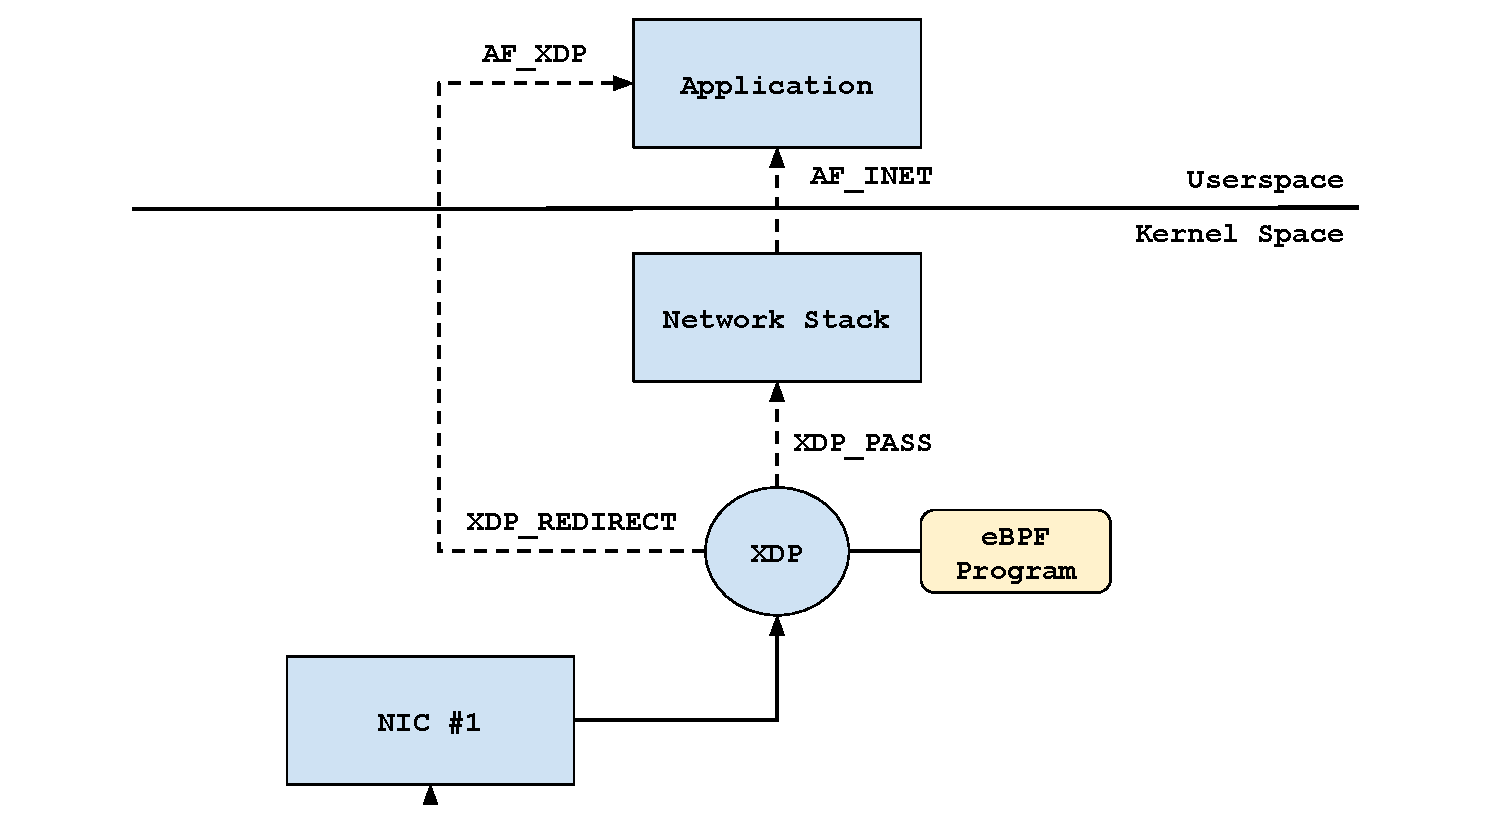
\includegraphics[width=.90\textwidth]{pics/xdp-actions-af-xdp.pdf}
        \nocite{af_xdp_image}
        \label{fig1}
    \end{figure}
\end{frame}

\section{AF\_XDP Primer}
\begin{frame}
    \begin{itemize}
        \item UMEM is a data buffer in userspace memory; it stores packets
        \item Packets be directly copied into the UMEM from the NIC (i.e. zero-copy or zc)
        \item Alternatively, packets can be copied into kernel memory first and later into the UMEM
    \end{itemize}
    \begin{figure}
        \centering
        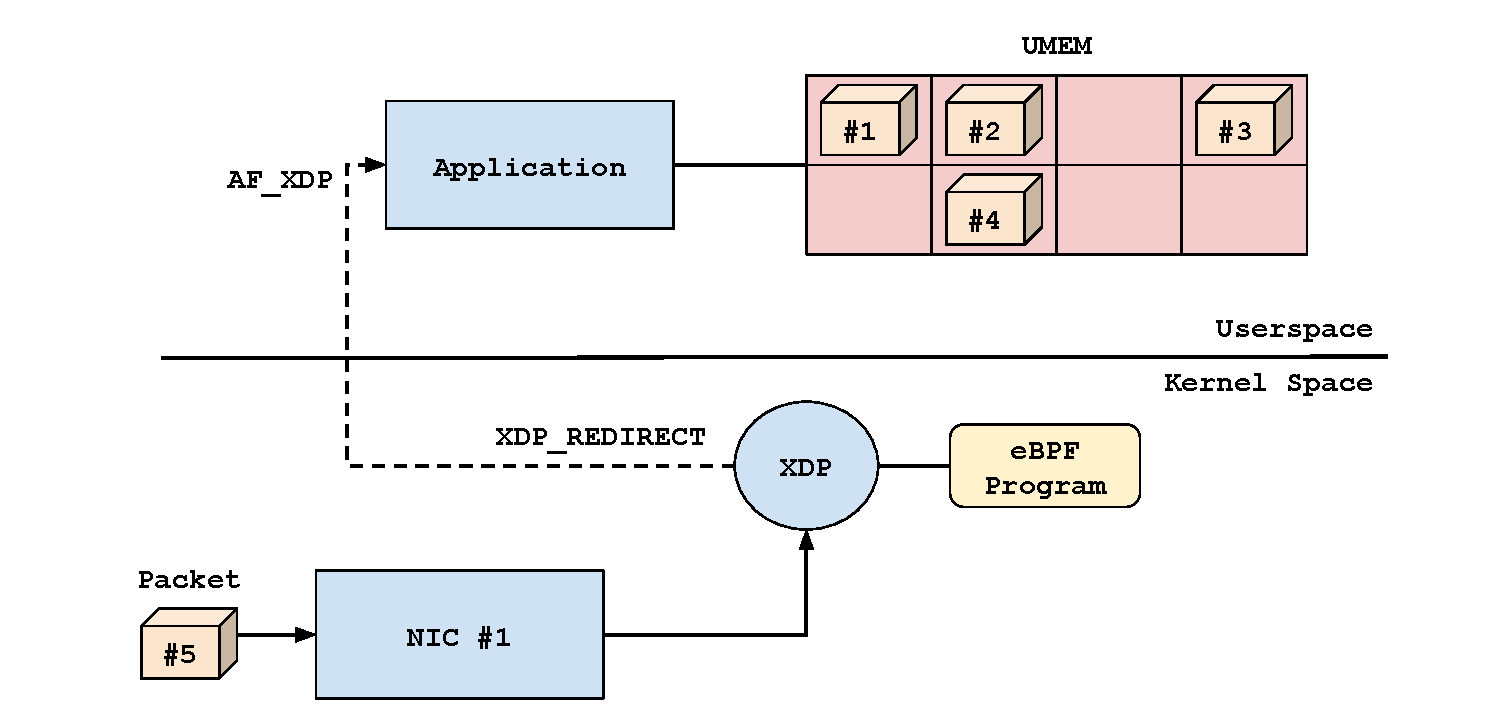
\includegraphics[width=.90\textwidth]{pics/UMEM-region.pdf}
    \end{figure}
\end{frame}

% - Then give brief introductions to XDP and QUIC
%     - QUIC is an L4 protocol, similar to TCP, which runs in userspace. This means packets must go through the network stack to reach the protocol. The network stack may waste cycles adding metadata to your packet that you don't need. AF_XDP allows you to get the packet at the earliest possible point.
%     - AF_XDP lets you skip the Linux network stack
%     - XDP is a hook in the kernel which allows you to process handle a packet at the 
%     earliest possible time. It is a _native_ kernel feature, which means you can use
%     it for many possible applications.

\section{Additional Optimizations}
\begin{frame}
    \frametitle{recvmmsg(2)}
    \begin{figure}
        \centering
        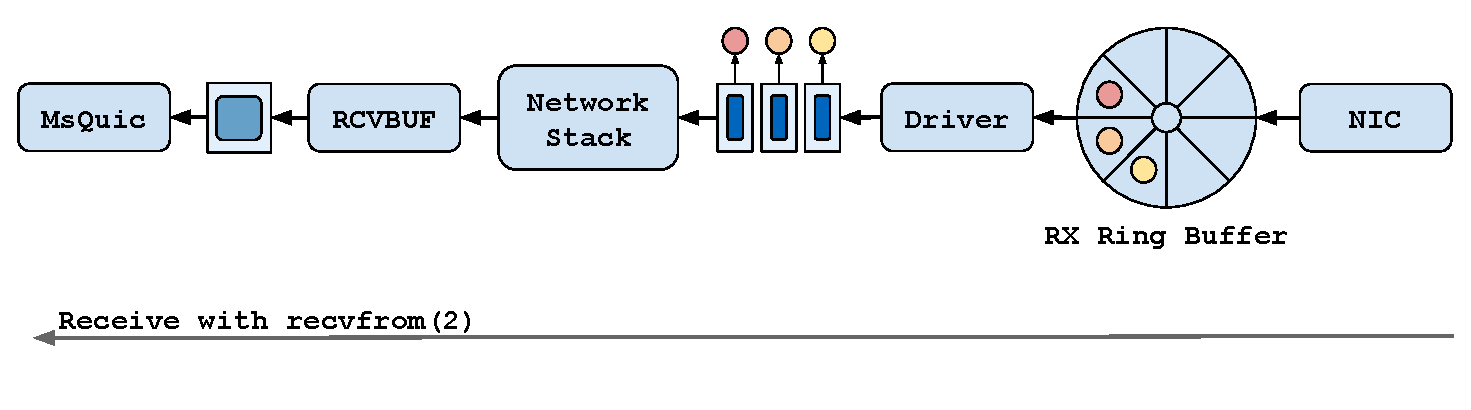
\includegraphics[width=.90\textwidth]{pics/diag-recvfrom(2)v2.pdf}
    \end{figure}
    \pause % this basically creates two slides.
    \begin{figure}
        \centering
        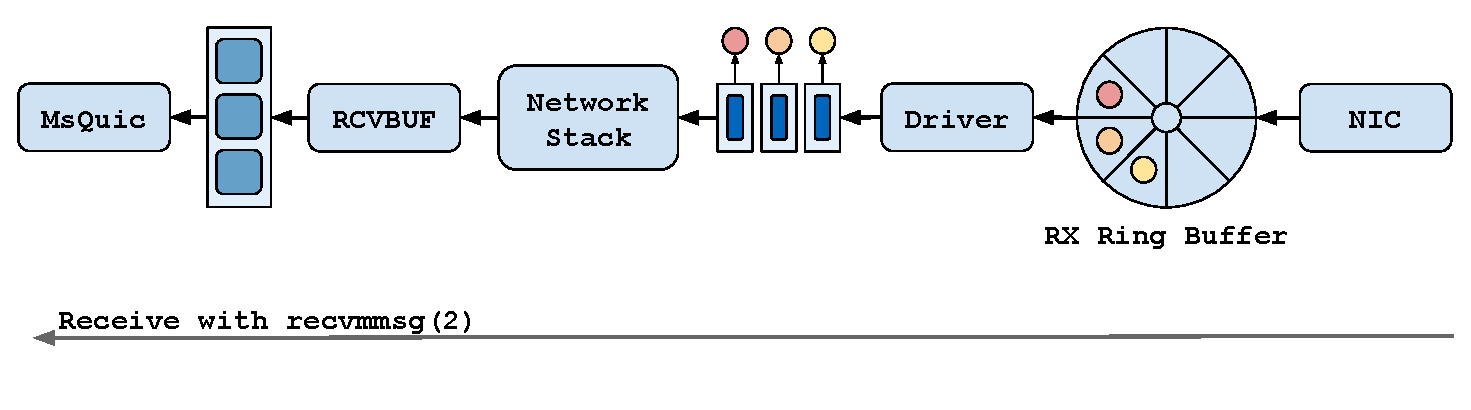
\includegraphics[width=.90\textwidth]{pics/diag-recvmmsg(2)v2.pdf}
    \end{figure}

\end{frame}

\section{Additional Optimizations}
\begin{frame}
    \frametitle{Generic Receive Offload (GRO)}
    \begin{figure}
        \centering
        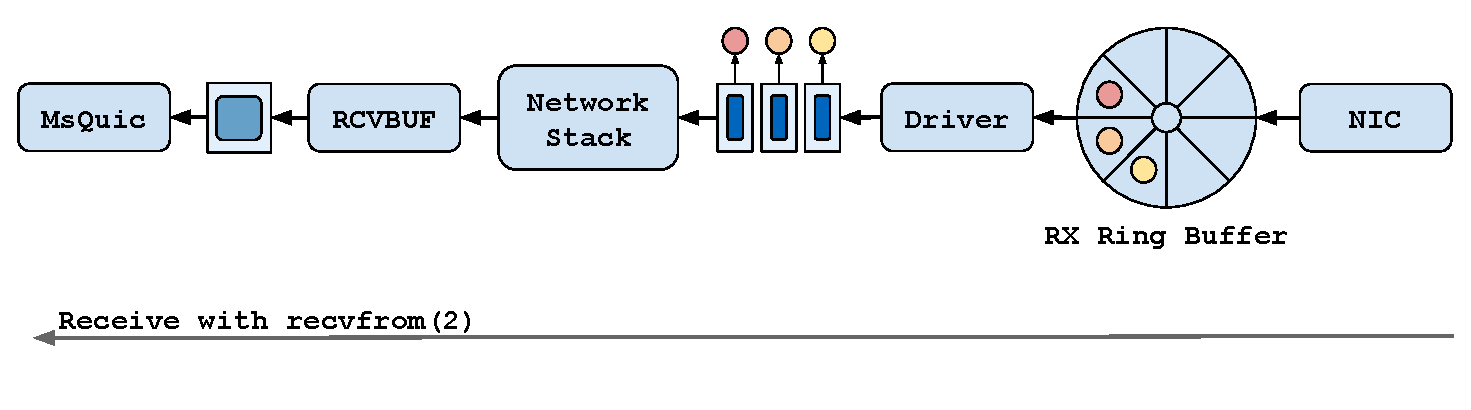
\includegraphics[width=.90\textwidth]{pics/diag-recvfrom(2)v2.pdf}
    \end{figure}
    \begin{figure}
        \centering
        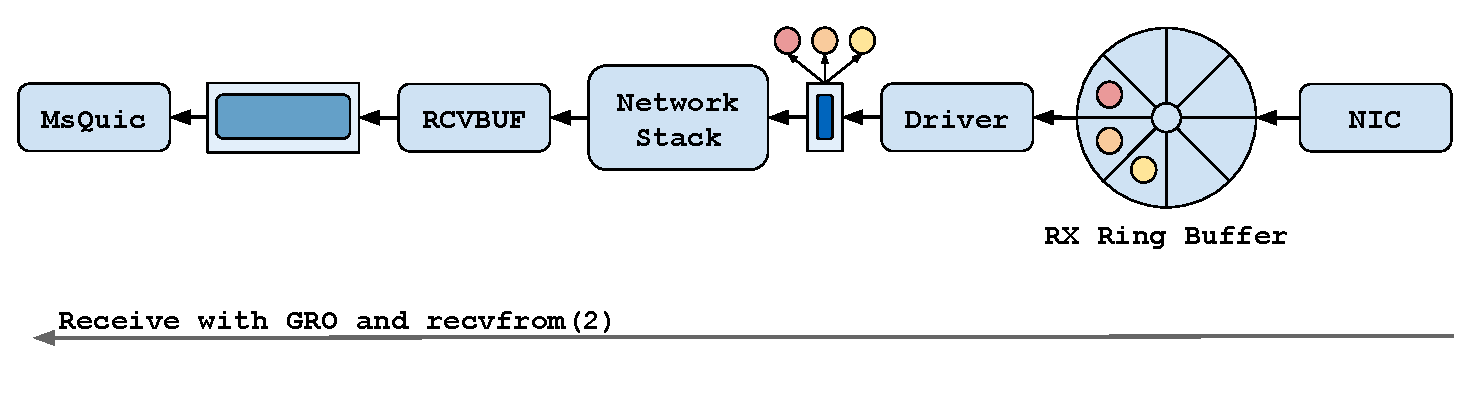
\includegraphics[width=.90\textwidth]{pics/diag-grov2.pdf}
    \end{figure}
\end{frame}

\section{Additional Optimizations}
\begin{frame}
    \frametitle{GRO + recvmmsg(2)}
    \begin{figure}
        \centering
        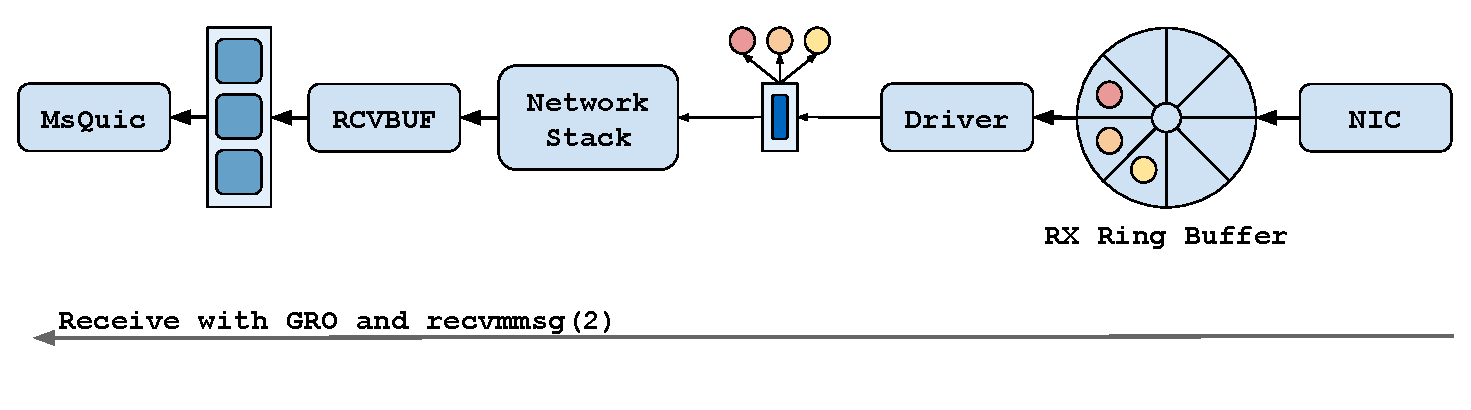
\includegraphics[width=.90\textwidth]{pics/diag-recvmmsg(2)+grov2.pdf}
    \end{figure}
    \pause
    \begin{itemize}
        \item A similar optimization exists for sending:
        \begin{itemize}
            \item Generic Segmentation Offload (GSO)
            \item sendmmsg(2)
        \end{itemize}
    \end{itemize}
\end{frame}

% \item recvmmsg(2) system call receives multiple messages from a socket in a single call, which can be more efficient than making multiple recvfrom(2) calls.
% \item GRO combines network packets into a single larger one, reducing the number of packets the CPU has to process


\section{Approach}
\begin{frame}
    \frametitle{Goodput}
    \begin{itemize}
        \item Patch MsQuic\footnote{https://github.com/microsoft/msquic} to support AF\_XDP
        \item Run throughput tests in a client-server topology
        \item 20 iterations with 8GB file size using weak (Dogecoin) and strong (Opulous) CPU setups:
        \begin{itemize}
            \item Dogecoin: \emph{Intel Xeon D-1518 @ 2.20GHz 4-core} CPU, 32 GB of RAM, and \emph{Intel X552 10 GbE SFP+} NICs, over a 10G link\footnote{Additionally, ixgbe driver (version 6.1.0-17-amd64) was used}
            \item Opulous: \emph{AMD EPYC 9354 @ 3.25 GHz 32-core} CPU, 768 GB of RAM, and \emph{Mellanox ConnectX-6} NICs over a 100G link\footnote{Additionally, mlx5\_core driver (version 6.1.0-17-amd64) was used}
        \end{itemize}        
    \end{itemize}
    \begin{figure}
        \centering
        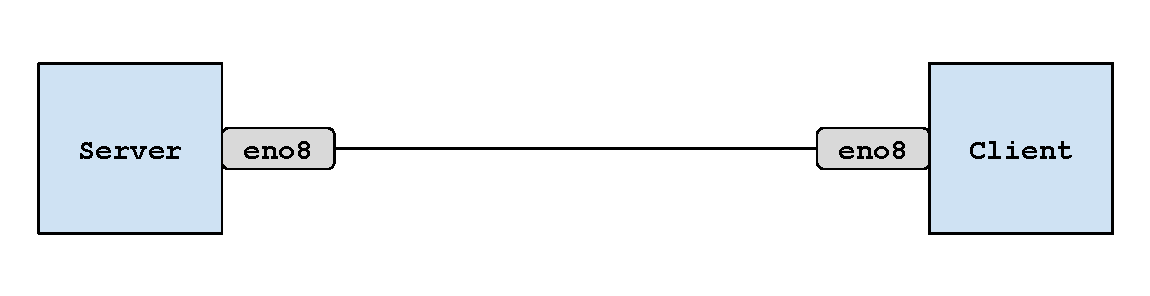
\includegraphics[width=.75\textwidth]{pics/throughput-topology.pdf}
        \label{fig3}
    \end{figure}
\end{frame}

\section{XDP Hook Points}
\begin{frame}
    \begin{itemize}
        \item Two different XDP hook points: \texttt{XDP\_DRV} and \texttt{XDP\_SKB}
        \item \texttt{XDP\_SKB} requires additional processing over \texttt{XDP\_DRV}
    \end{itemize}
    \begin{figure}
        \centering
        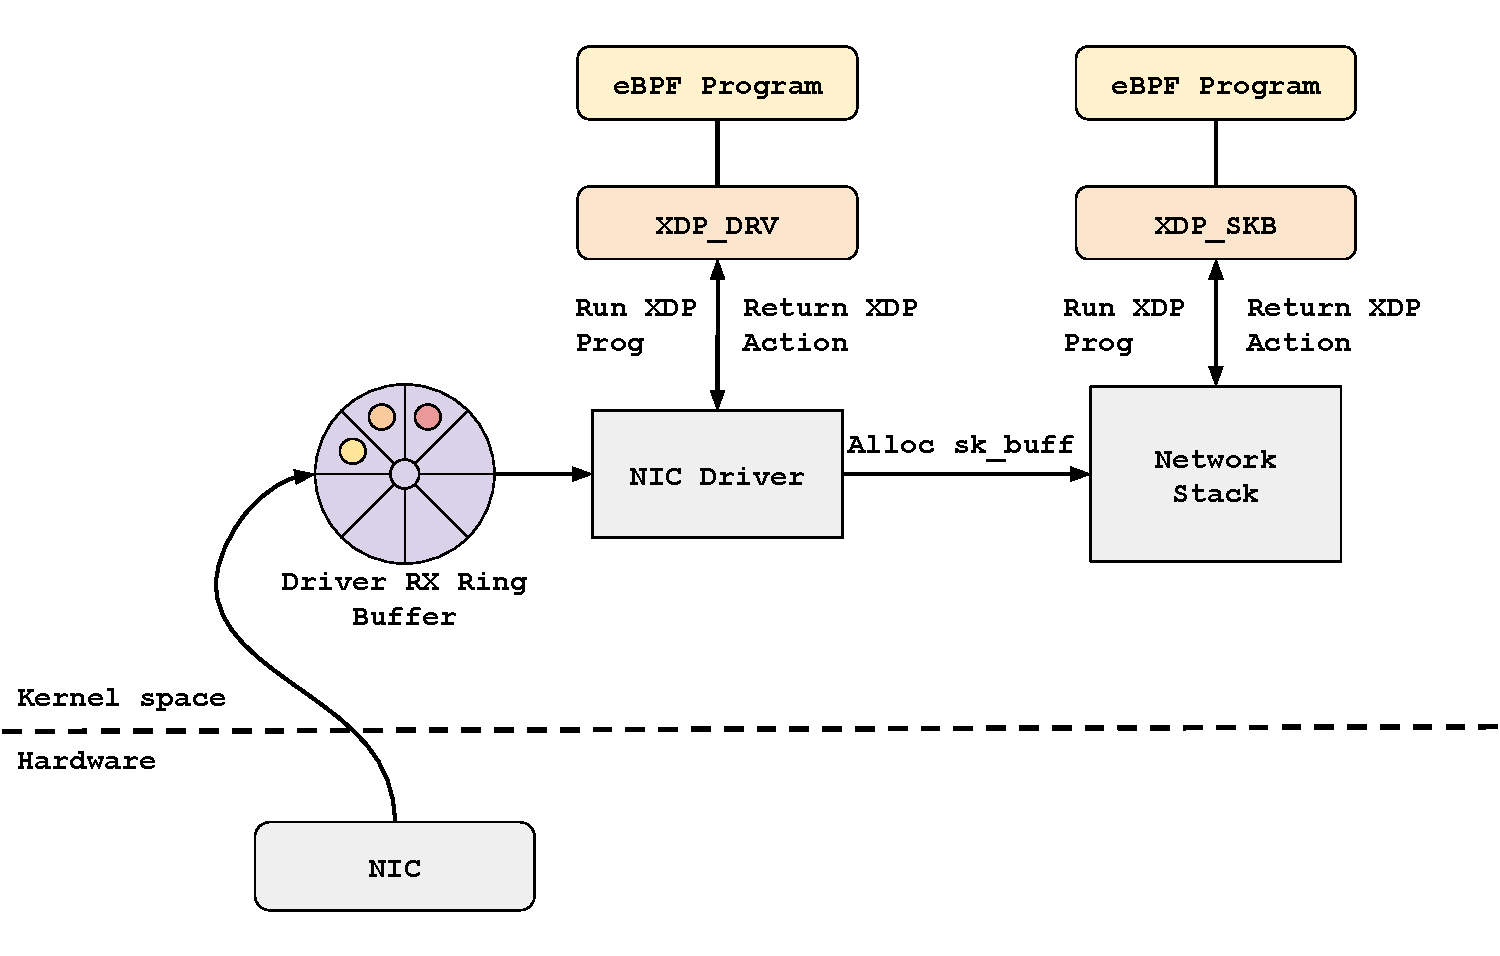
\includegraphics[width=.75\textwidth]{pics/xdp-receive-path3.pdf}
    \end{figure}
\end{frame}

\section{XDP Types}
\begin{frame}
    \begin{itemize}
        \item Three XDP types: \texttt{XDP\_SKB}, \texttt{XDP\_DRV}, and \texttt{XDP\_DRV+zc} (i.e. zero-copy)
        \item For \texttt{XDP\_DRV+zc}, packet is copied by NIC directly into UMEM region
        \item For \texttt{XDP\_SKB} and \texttt{XDP\_DRV}, an intermediate copy into kernel memory is required
        \item A similar process exists for sending
    \end{itemize}
    \begin{figure}
        \centering
        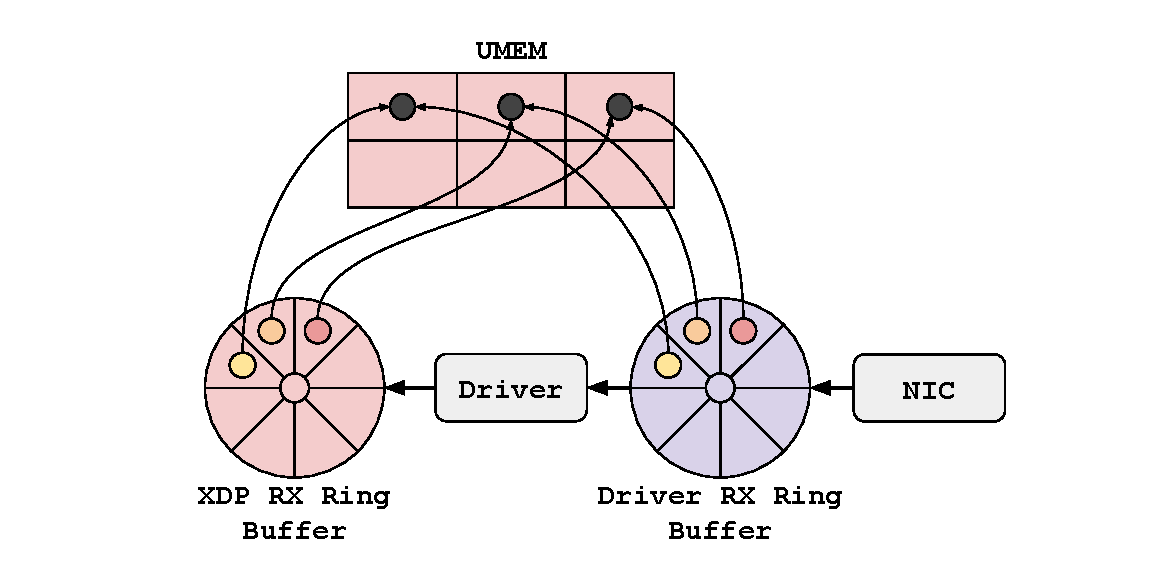
\includegraphics[width=.75\textwidth]{pics/xdp-zerocopy.pdf}
    \end{figure}
\end{frame}

\section{Measurements}
\begin{frame}
    \frametitle{AF\_XDP on the Server (Dogecoin)}
    \begin{itemize}
        \item \texttt{XDP\_DRV+zc} exhibits higher goodput than substitutes but remains lower than \texttt{sendmmsg+GSO}
        \item \texttt{GSO} makes the difference within the default datapath
    \end{itemize}
    \begin{figure}
        \centering
        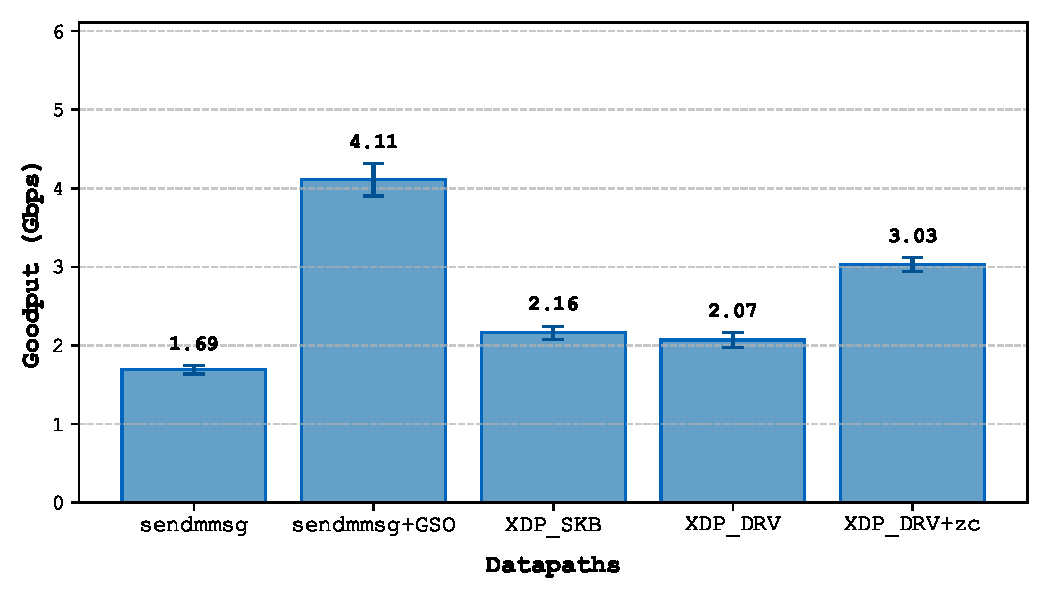
\includegraphics[width=.75\textwidth]{pics/dogecoin-server-goodput.pdf}
        \label{fig4}
    \end{figure}
\end{frame}

\section{Measurements}
\begin{frame}
    \frametitle{AF\_XDP on the Server, continued}
    \begin{itemize}
        \item System CPU usage for \texttt{XDP\_SKB} and \texttt{XDP\_DRV} higher than \texttt{XDP\_DRV+zc}
        \item We used a perf trace to pinpoint the increased time spent copying data from the UMEM to kernel memory
    \end{itemize}
    \begin{figure}
        \centering
        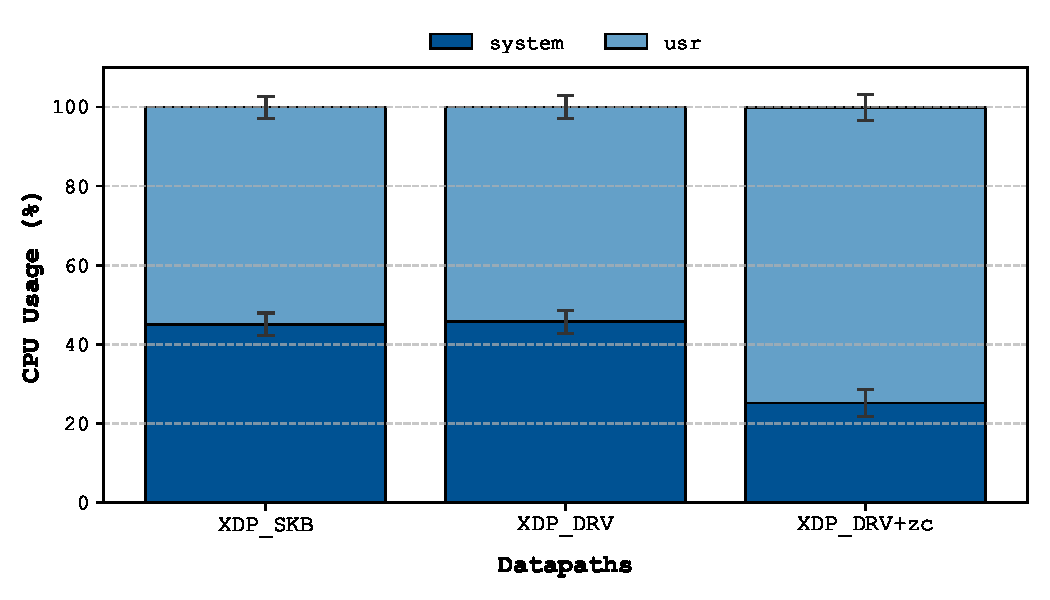
\includegraphics[width=.75\textwidth]{pics/pidstat-stacked-plot-server.pdf}
    \end{figure}
\end{frame}

\section{Measurements}
\begin{frame}
    \frametitle{AF\_XDP on the Client (Dogecoin)}
    \begin{itemize}
        \item Surprisingly, the XDP alternatives are no longer statistically significant from each other
        \item Talk about large \texttt{XDP\_SKB} std dev. here?
    \end{itemize}
    \begin{figure}
        \centering
        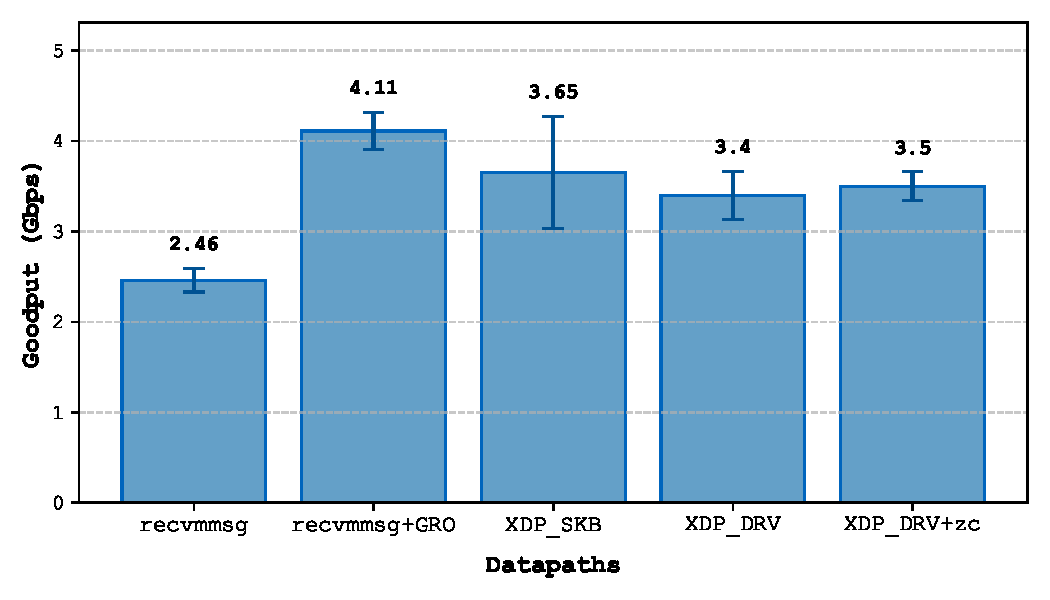
\includegraphics[width=.75\textwidth]{pics/dogecoin-client-goodput.pdf}
        \label{fig5}
    \end{figure}
\end{frame}

\section{Measurements}
\begin{frame}
    \frametitle{RX Batch Sizes with AF\_XDP on the Client (Dogecoin)}
    \begin{itemize}
        \item Goodput increases as RX batch size increases until 32
        \item The bottleneck changes; MsQuic must no longer wait for packets and instead spends its time on processing
    \end{itemize}
    \begin{figure}
        \centering
        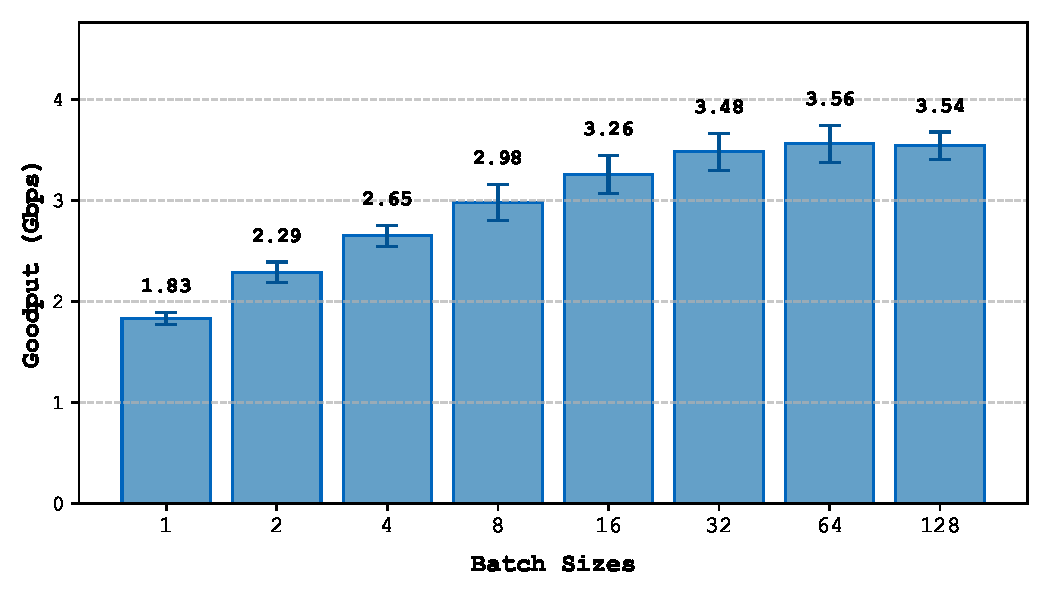
\includegraphics[width=.75\textwidth]{pics/dogecoin-batch-size.pdf}
        \label{fig6}
    \end{figure}
\end{frame}

\section{Approach}
\begin{frame}
    \frametitle{NIC-to-Userspace Packet Traversal Time}
    \begin{itemize}
        \item Sync NICs and system times using Precision Time Protocol (PTP)\footnote{https://github.com/richardcochran/linuxptp}
        \item 1 iteration with 128MB file size using Dogecoin\footnote{Dogecoin: \emph{Intel Xeon D-1518 @ 2.20GHz 4-core} CPU, 32 GB of RAM, and \emph{Intel X552 10 GbE SFP+} NICs, using \emph{ixgbe driver} (version 6.1.0-17-amd64) over a 10 Gbase link.}
        \item Generates more than 100k NIC-to-Userspace packet time differences
        \item Poor documentation and integration into QIR was a difficult and length process
    \end{itemize}
    \begin{figure}
        \centering
        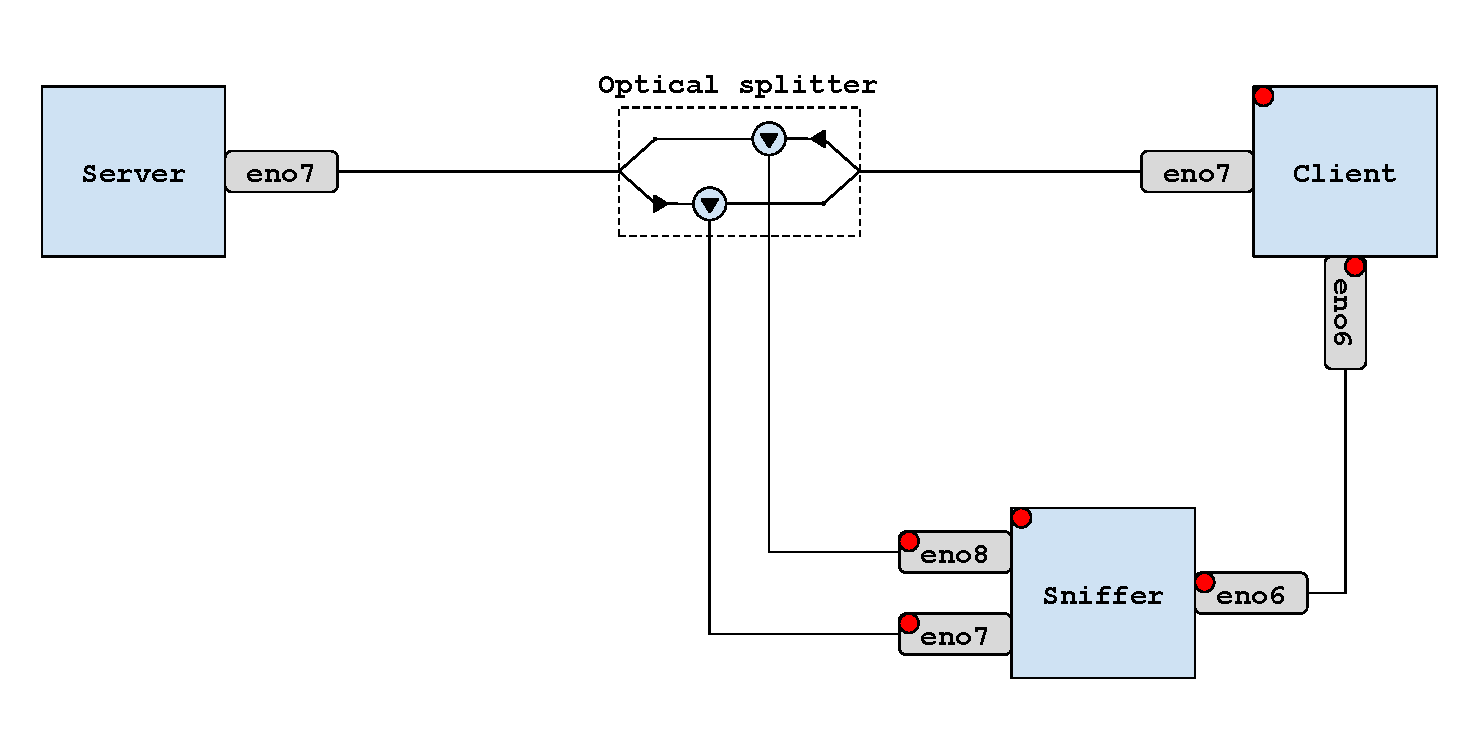
\includegraphics[width=.75\textwidth]{pics/ptp-topology2v2.pdf}
        \label{fig3}
    \end{figure}
\end{frame}

\section{Measurements}
\begin{frame}
    \begin{itemize}
        \item XDP and default datapath NIC-to-userspace times mostly remain in parity
        \item The long tail in the non-XDP case is likely due to additional queues in the receive path
    \end{itemize}
    \begin{figure}
        \centering
        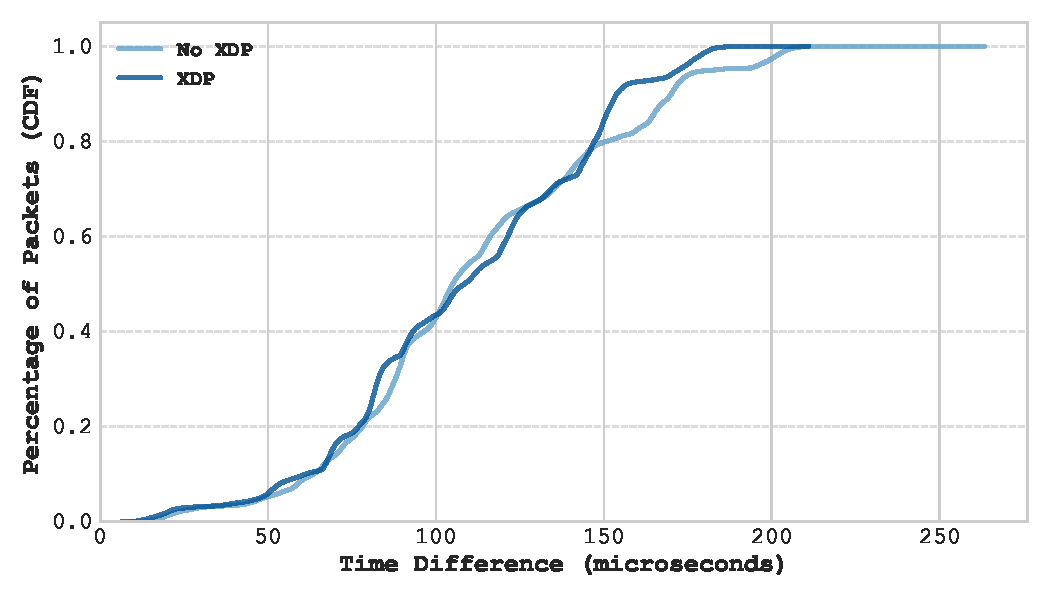
\includegraphics[width=.75\textwidth]{pics/ptp-log-cdf.pdf}
    \end{figure}
\end{frame}

\section{Related Work}
\begin{frame}
    \begin{itemize}
        \item DPDK\footnote{https://www.dpdk.org/}\nocite{dpdk} enables kernel bypass and allows application to connect directly to the NIC, reducing kernel overhead
        \item lxin-quic\footnote{https://github.com/lxin/quic}\nocite{lxin_quic} brings QUIC into the kernel, reducing context switches and copying between kernel and userspace
        \item \textit{QUIC Performance Improvements Using Socket Optimizations and Kernel Bypass}\footnote{Späth, J. QUIC performance improvements using socket optimizations and kernel bypass. Master’s thesis, TU Munich, 2023.}\nocite{spaeth2023} investigates methods to improve QUIC performance by means
        of patching MsQuic with DPDK and using socket optimizations
    \end{itemize}
    % \begin{figure}
    %     \centering
    %     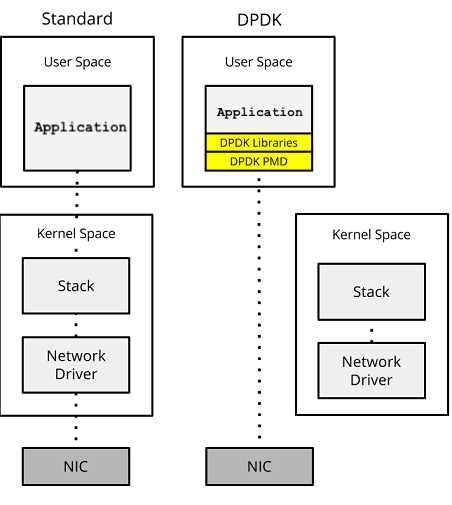
\includegraphics[width=.75\textwidth]{pics/dpdk.png}
    %     \label{fig81}
    %     \nocite{donato2018dpdk}
    % \end{figure}
\end{frame}

\section{QUIC Datapaths}
\begin{frame}
    \begin{figure}
        \centering
        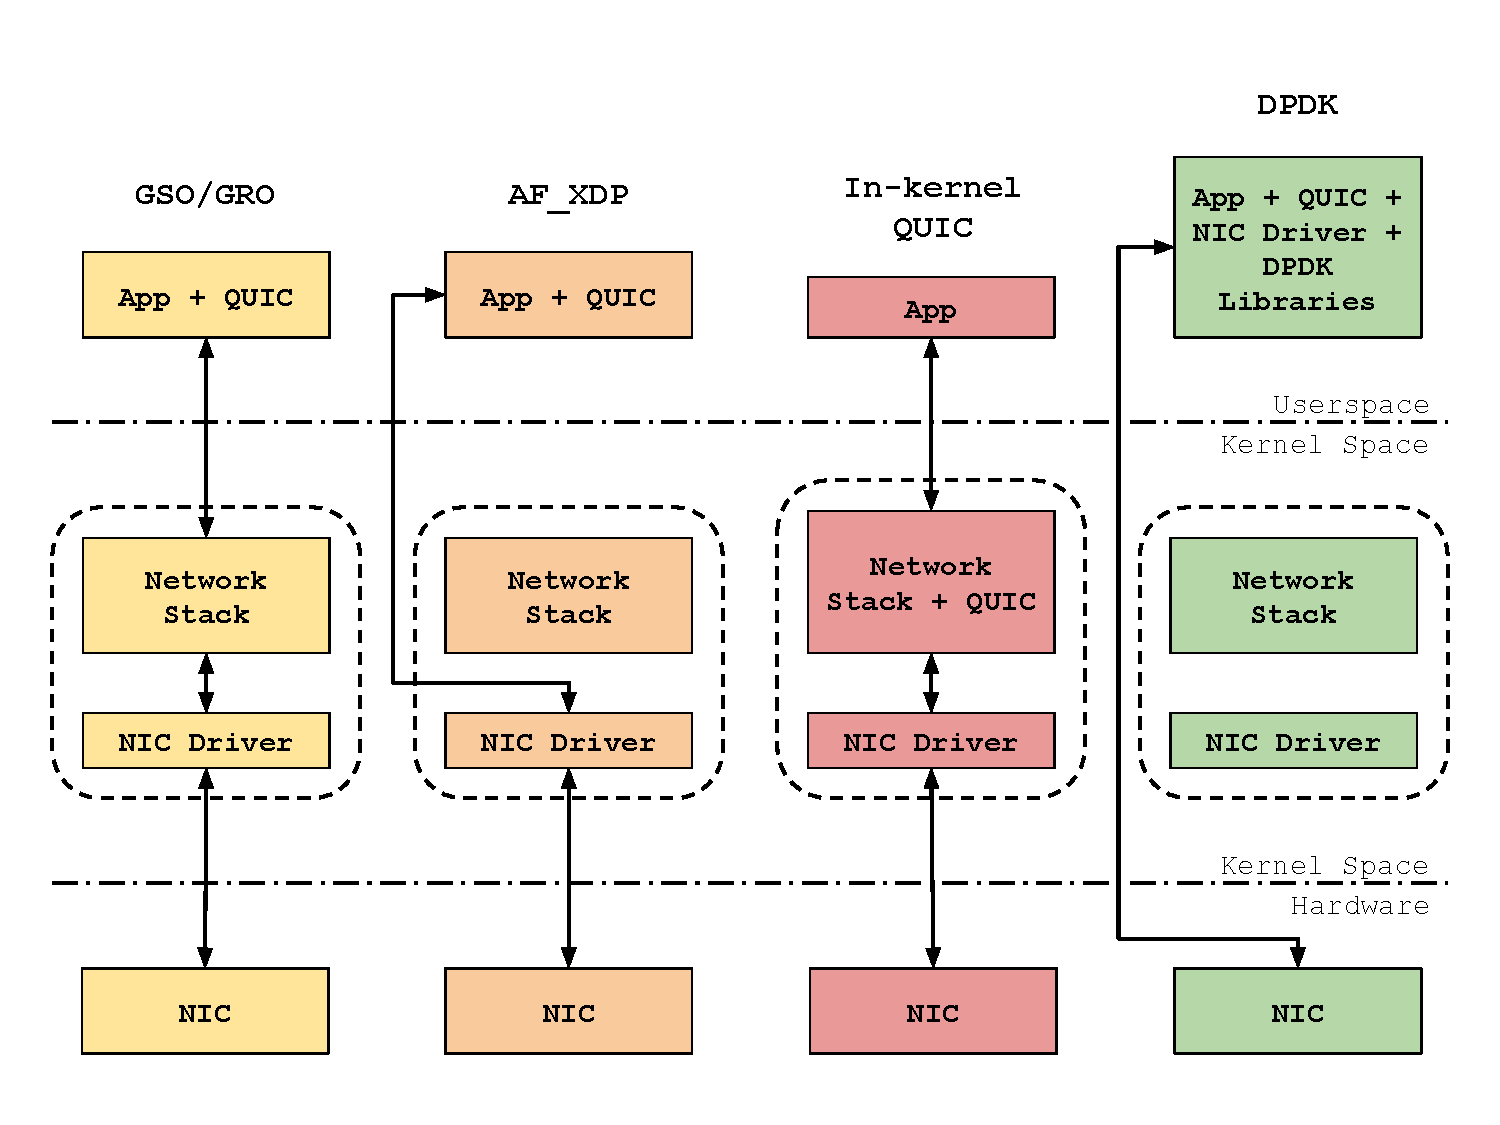
\includegraphics[width=.90\textwidth]{pics/QUIC-datapaths.pdf}
    \end{figure}
\end{frame}

\section{Taxonomy of QUIC Datapaths}
\begin{frame}
    \begin{table}[h]
    \small
    \centering
    \begin{tabular}{lcccc}
        \toprule
        \textbf{Metric} & \textbf{GSO/GRO} & \textbf{AF\_XDP} & \textbf{In-kernel QUIC} & \textbf{DPDK} \\
        \midrule
        \textbf{Impl. Complexity} & Low & High & High & High \\
        \textbf{Standardized APIs} & \yes & \no & \yes & \no \\
        \textbf{Kernel Integration} & High & Medium & High & Low \\
        \textbf{NIC Sharing} & \yes & \yes & \yes & \no \\
        \textbf{Hardware Agnostic} & High & High* & High & Low \\
        \textbf{Maturity} & High & Medium & Low & High\\
        \textbf{Tooling} & High & High & High & Medium \\
        \textbf{Privileged Access} & \yes & \yes & \yes & \yes \\
        \bottomrule
    \end{tabular}
\end{table}
\end{frame}

% \section{Optimization}
% \begin{frame}
%     Optimized datapath initialization time (3s in perf trace) by configuring UMEM for a single queue on one interface
%     \begin{figure}
%         \centering
%         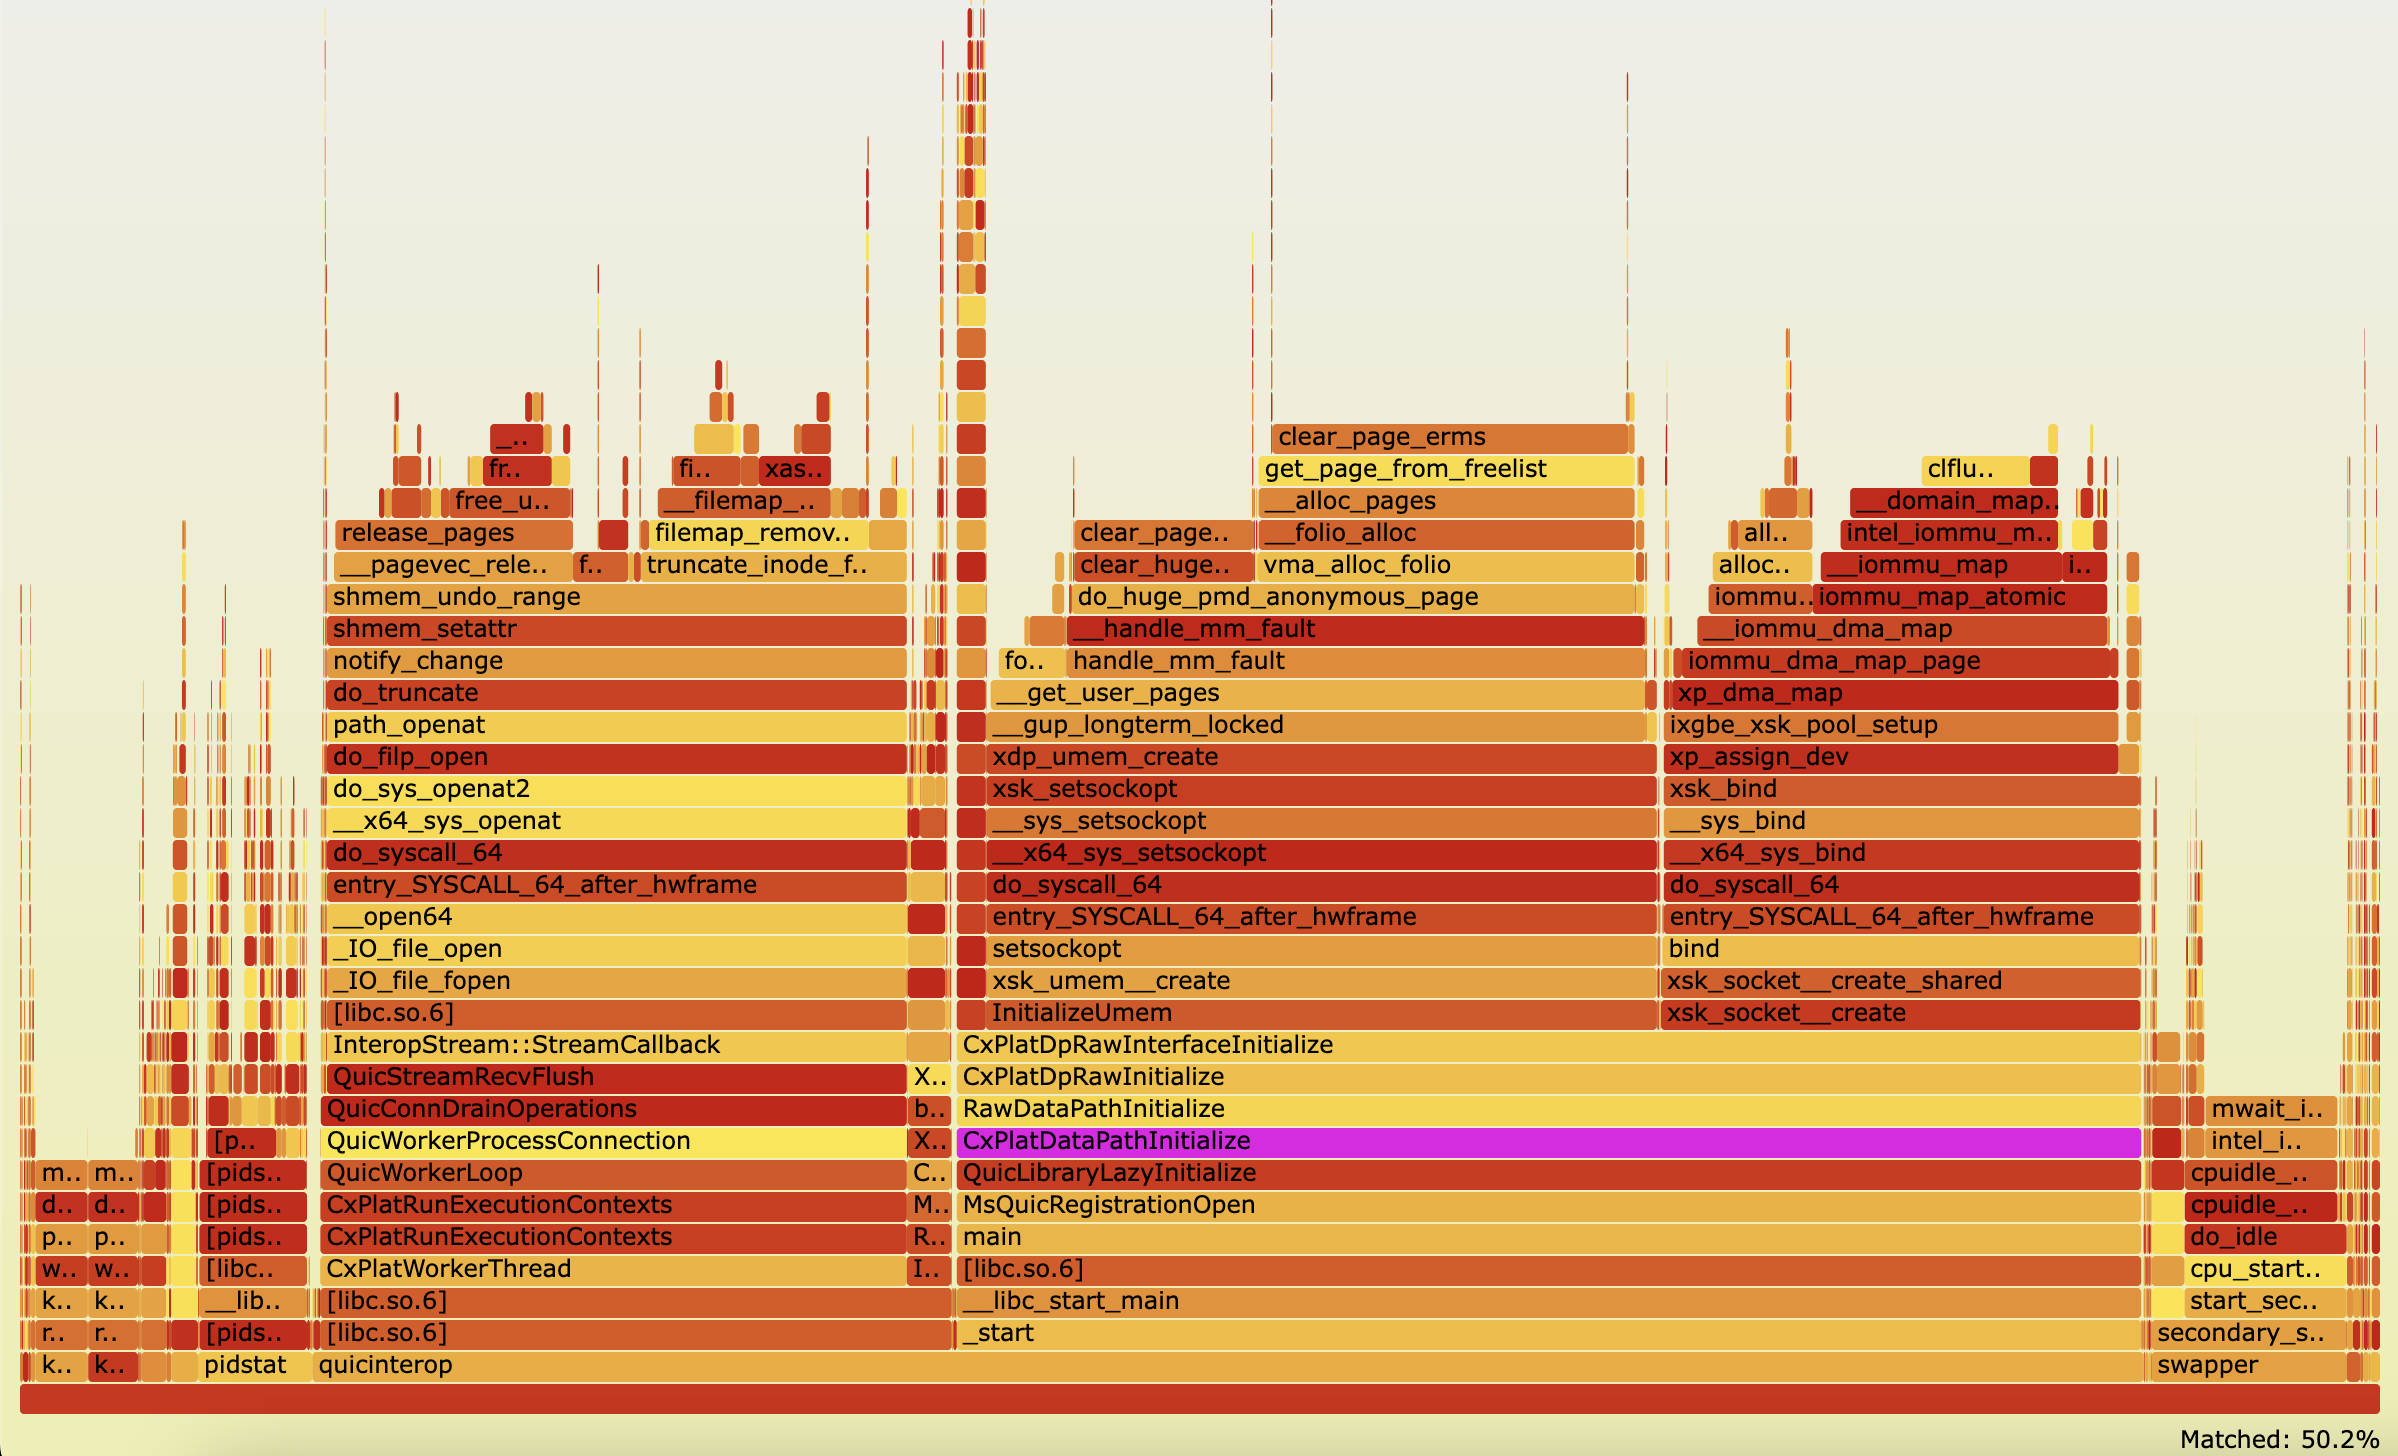
\includegraphics[width=1\textwidth]{pics/DataPathInitialize_beforeOpt.png}
%         \label{fig31}
%     \end{figure}
% \end{frame}

% \section{Optimization}
% \begin{frame}
%     \begin{figure}
%         \centering
%         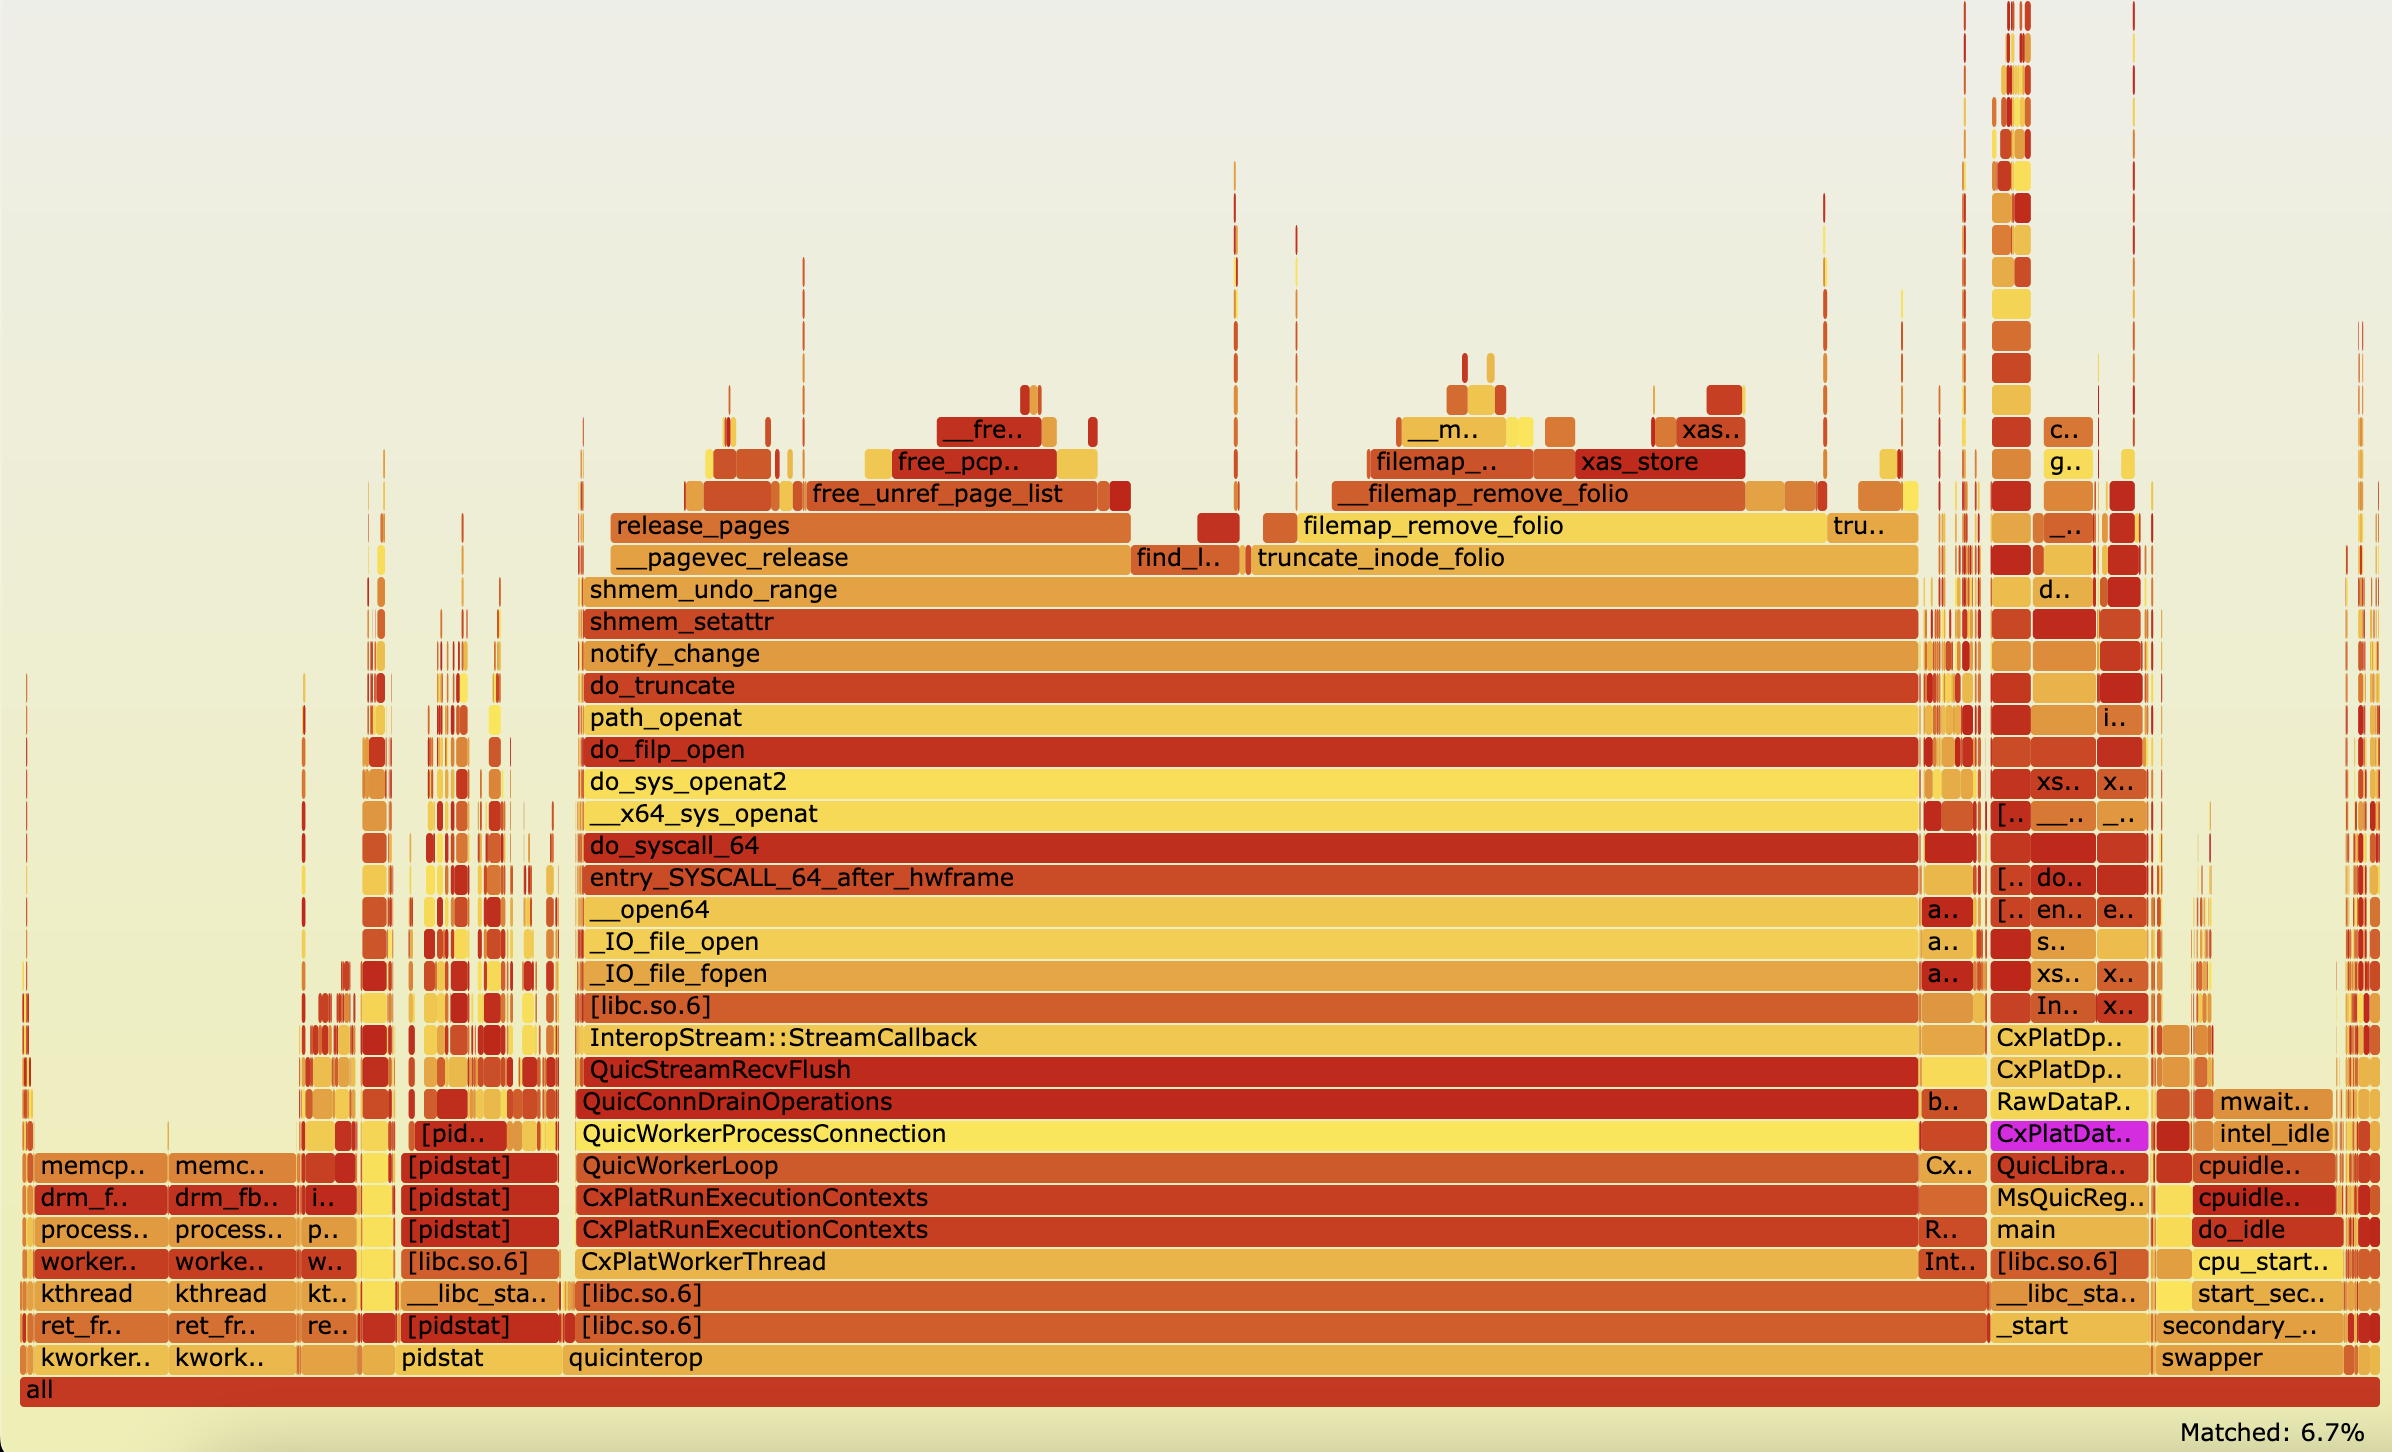
\includegraphics[width=1\textwidth]{pics/DataPathInitialize_afterOpt.png}
%         \label{fig32}
%     \end{figure}
% \end{frame}

% \section{GRO for XDP}
% \begin{frame}
%     \begin{itemize}
%         \item Fragmentation with XDP now supported by some NIC drivers\footnote{https://github.com/torvalds/linux/commit/f52ac7028bec22e925c8fece4f21641eb13b4d6f}\nocite{torvalds2021xdp}
%         \item \texttt{rx-gro-hw} with XDP\_DRV or GRO with XDP\_SKB when HW offload not available
%     \end{itemize}
%     \begin{figure}
%         \centering
%         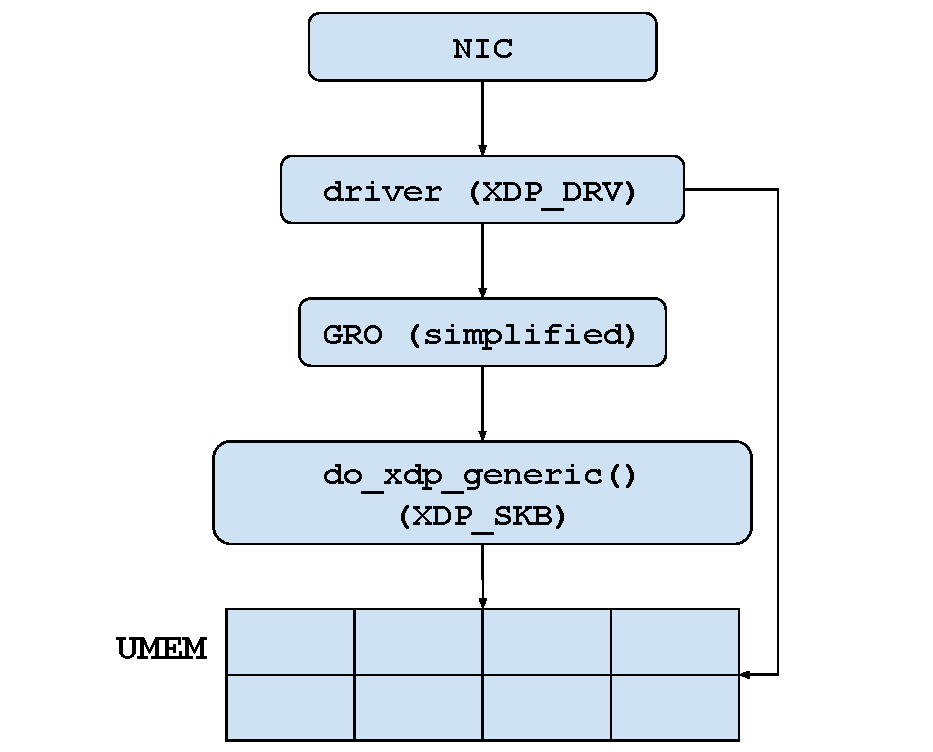
\includegraphics[width=.60\textwidth]{pics/gro_offload_simplified.pdf}
%         \label{fig8}
%     \end{figure}
% \end{frame}

\section{Conclusion}
\begin{frame}
    \begin{itemize}
        \item To what extent can we increase QUIC performance by using XDP in a trivial way? Is there optimization potential?
        \begin{itemize}
            \item AF\_XDP is not able to achieve a higher goodput over the optimized default datapath
            \item Also, AF\_XDP NIC-to-userspace times remain consistent with the default datapath
            \item However, optimization potential exists
        \end{itemize}
    \end{itemize}
    \begin{itemize}
        \item Can a taxonomy be created for QUIC optimizations, categorized by:
        \begin{itemize}
            \item Implementation complexity
            \item Performance improvement potential
            \item Unwanted side effects
            \item Privilege level usage
            \item Deployment
        \end{itemize}
    \end{itemize}
    \begin{center}
        \yes\ Yes, each datapath offers its unique set of tradeoffs
    \end{center}
\end{frame}

\section{Future Work}
\begin{frame}
    \begin{itemize}
        \item Enable GRO for AF\_XDP, for which driver support has been increasing~\cite{xdp_multibuff_2019}
        \item Increase the TX ring batch size from its default of 1, which may offer similar speedups as seen in the RX batch size case
        \item Perform throughput and latency measurements across all QUIC datapaths on the same testbed
    \end{itemize}
\end{frame}

\section{Appendix}
\begin{frame}
    \frametitle{AF\_XDP on the Server (Opulous)}
    \begin{figure}
        \centering
        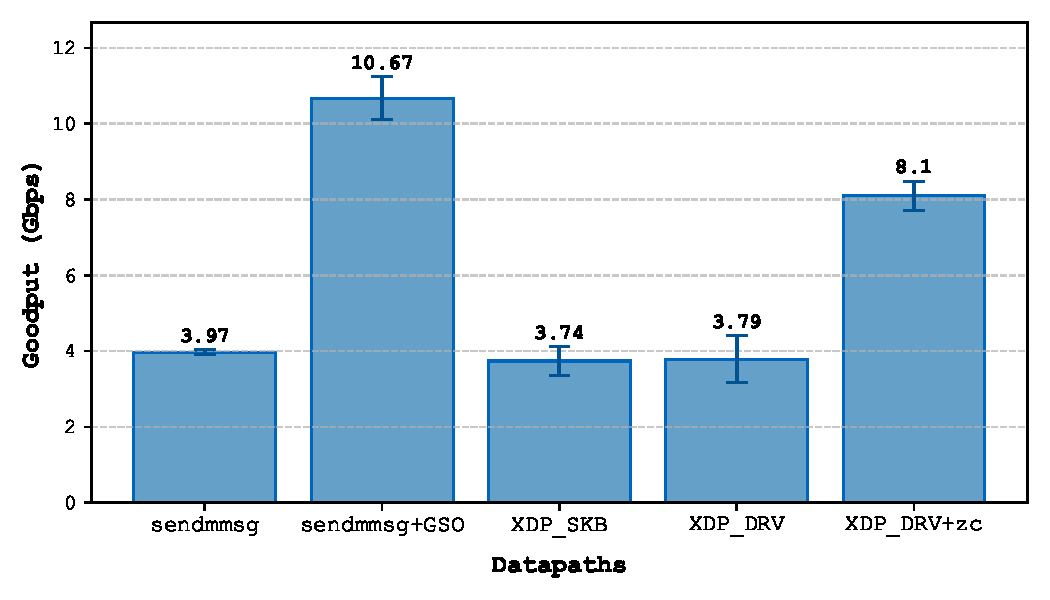
\includegraphics[width=.75\textwidth]{pics/opulous-server-goodput.pdf}
    \end{figure}
\end{frame}

\section{Appendix}
\begin{frame}
    \frametitle{AF\_XDP on the Client (Opulous)}
    \begin{figure}
        \centering
        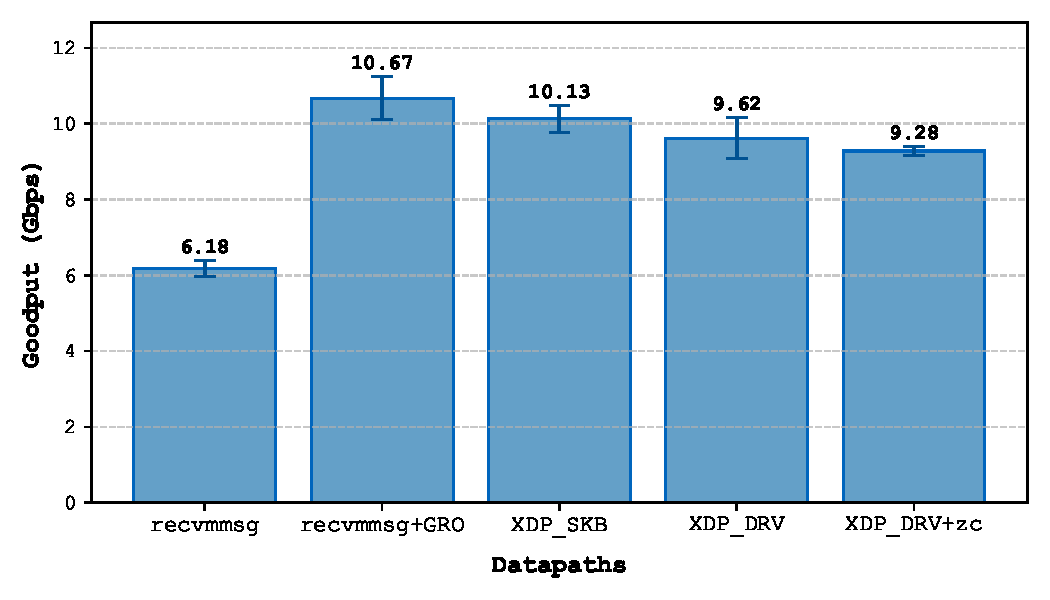
\includegraphics[width=.75\textwidth]{pics/opulous-client-goodput.pdf}
    \end{figure}
\end{frame}

\section{Appendix}
\begin{frame}
    \frametitle{XDP Types: XDP\_SKB}
    \begin{itemize}
        \item Packet is copied by NIC into kernel memory and an sk\_buff is allocated
        \item Packet is copied from kernel memory into the UMEM region
    \end{itemize}
    \begin{figure}
        \centering
        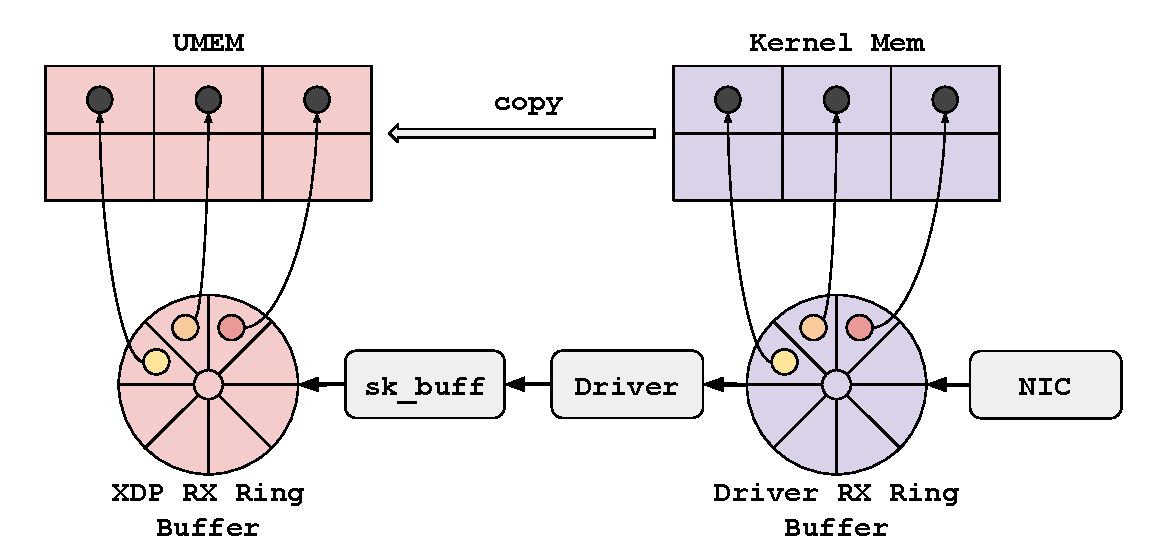
\includegraphics[width=.75\textwidth]{pics/skb-mode.pdf}
    \end{figure}
\end{frame}

\section{Appendix}
\begin{frame}
    \frametitle{XDP Types: XDP\_DRV}
    \begin{itemize}
        \item Packet is copied by NIC into kernel memory; no sk\_buff this time
        \item Packet is copied from kernel memory into the UMEM region 
    \end{itemize}
    \begin{figure}
        \centering
        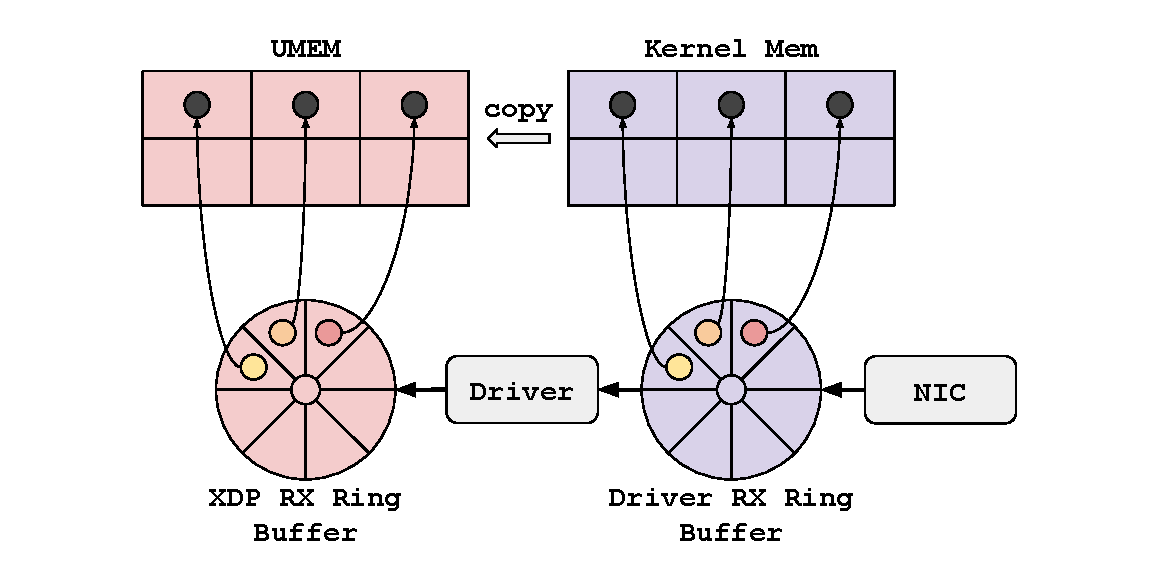
\includegraphics[width=.75\textwidth]{pics/no-xdp-zerocopy.pdf}
    \end{figure}
\end{frame}

% \section{FEC Primer}
% \begin{frame}
%     % \frametitle{What is FEC}
%     \begin{itemize}
%         \item Protect QUIC stream and datagram frames
%         \item Trade bandwidth for reliability
%         \item Send redundant data
%         \item Reconstruct lost information with repair symbols
%     \end{itemize}
%     \begin{figure}
%         \centering
%         \includegraphics[width=.75\textwidth]{pics/source_repair2}
%         \label{fig2}
%     \end{figure}
% \end{frame}

% \section{FEC Primer}
% \begin{frame}
%     % \frametitle{What is FEC}
%     \textbf{Many possible coding schemes}
%     \begin{itemize}
%         \item Block Codes
%         \begin{itemize}
%             \item XOR
%             \item Reed-Solomon
%         \end{itemize}
%         \item Convolutional Codes
%         \begin{itemize}
%             \item Sliding Window Random Linear Codes (RLC)
%         \end{itemize}
%     \end{itemize}
%     \begin{figure}
%         \centering
%         \includegraphics[width=.75\textwidth]{pics/xor-encoding-scheme}
%         \label{fig3}
%     \end{figure}
% \end{frame}

% \section{Goals}
% \begin{frame}
%     % \frametitle{What is FEC}
%     \begin{itemize}
%         \item Interpret and implement IETF draft \texttt{michel-quic-fec} \cite{michel-quic-fec-01} in quic-go
%         \item Find flaws within specification and communicate them back to author
%         \item Measure performance under different network conditions
%         \item Interoperate with other implementations
%     \end{itemize}
% \end{frame}

% \section{Approach}
% \begin{frame}
% \textbf{Extend QUIC send API}
%     \begin{itemize}
%         \item FEC-protected streams and datagrams
%         \item Logic for encoding schemes
%         \item Handlers for source and repair symbols
%     \end{itemize}
% \textbf{Measurements with pos tesbed}
%     \begin{itemize}
%         \item \texttt{netem} file download scenario with client-server architecture
%     \end{itemize}
% \end{frame}

% \section{Architecture}
% \begin{frame}
%     \frametitle{QUIC + FEC}
%     \begin{figure}
%         \centering
%         \includegraphics[width=.75\textwidth]{pics/quic-fec}
%         \label{fig5}
%         \nocite{quic_plus_fec}
%     \end{figure}
% \end{frame}

% \section{Related Work}
% \begin{frame}
%     \begin{itemize}
%         \item FlEC \cite{9861377} and PQUIC \cite{10.1145/3341302.3342078} are past implementations of QUIC + FEC
%         \item Draft \texttt{michel-quic-fec} (i.e. QUIRL) more performant in real-life networks
%     \end{itemize}
%     \begin{figure}
%         \centering
%         \includegraphics[width=.75\textwidth]{pics/quirl_vs2}
%         \label{fig6}
%         \nocite{francois-michel-phd-thesis}
%     \end{figure}
% \end{frame}

% \section{Challenges}
% \begin{frame}
% \textbf{Optimizing symbol generation and recovery}
% \begin{itemize}
%     \item CPU intensive
%     \item Within code hot-path; can slow down other operations
%     \item Refactoring difficult; would require changes to the entire database
% \end{itemize}
% \textbf{Limiting Memory Usage}
% \begin{itemize}
%     \item Unfinished blocks must keep symbols in memory
% \end{itemize}
% \textbf{Dealing with Complexity}
%     \begin{itemize}
%         \item \textasciitilde60k lines of code \cite{NET-2022-07-1_02}
%     \end{itemize}
% \end{frame}

% \section{Conclusion}
% \begin{frame}
%     \frametitle{and Next Steps}
%     \begin{itemize}
%         \item Implement XOR scheme \yes
%         \item Implement Reed-Solomon scheme
%         \item Complete measurement tests
%     \end{itemize}
%     \textbf{How to simulate real-life scenarios for more complex measurement tests?}
% \end{frame}

% \newcommand{\comment}[1]{}
% \comment{
% The talk has to be 15 minutes

% - Start off by talking about motiviation
%     - HTTP/3 commands 20\% of internet traffic worldwide and projected to grow? (this is why it's important)
%     - It has been shown to be slower than TCP on high-bandwidth networks (the problem)
%     - So we have to figure out a way to make it faster
%     - The biggest bottleneck in QUIC is packet I/O
%     - So let's explore one of the ways to reduce packet I/O -- i.e. XDP
% - Then give brief introductions to XDP and QUIC
%     - QUIC is an L4 protocol, similar to TCP, which runs in userspace. This means packets must go through the network stack to reach the protocol. The network stack may waste cycles adding metadata to your packet that you don't need. AF_XDP allows you to get the packet at the earliest possible point.
%     - AF_XDP lets you skip the Linux network stack
%     - XDP is a hook in the kernel which allows you to process handle a packet at the 
%     earliest possible time. It is a _native_ kernel feature, which means you can use
%     it for many possible applications.
% - Talk about related work
%     - DPDK is another specialized networking component, but it represents kernel-bypass,
%     which means that it can't take advantage of native kernel components. It also takes
%     control of the NIC, which means other applications can't use it *this is maybe not true anymore*.
% - Perhaps talk about challenges
% - Talk about next steps
%     - Maybe XDP frags?
%     - XDP checksum offload?
% }
